% ************************************************************************************************
% **************** Template para la elaboración del libro de Proyecto de Grado,*******************
% ******************** siguiendo los lineamientos establecidos por el ****************************
% ************* Decanato de Estudios Profesionales de la Universidad Simón Bolívar ***************
% *** "Normas para Redacción y Presentación del Libro Final del Proyecto de Grado y Pasantías" ***
% ***************** en la pág. web http://www.profesionales.usb.ve/es/node/4 *********************
% ************************************************************************************************

% ************************************************************************************************
% *** Versión: v1.0                                                                            ***
% *** Autor: Luis Pérez Bustos                                                                 ***
% *** Estudiante de Ingeniería Electrónica                                                     ***
% *** Fecha: 08/04/2017                                                                        ***                      
% *** Licencia: MIT License (c) 2017 Luis Perez Bustos                                         ***
% *** GitHub: https://github.com/lperezbustos/ProyectoDeGrado-Template-USB                     ***
% ************************************************************************************************

\documentclass[letterpaper,12pt,oneside,times,numbered,print,custommargin]{Clases/USB}

% El archivo README.md muestra información necesaria, por favor leerlo.

% ************************************** HEADER *****************************************
% ************************ Packages needed and some configurations **********************
% ***************************************************************************************

% ************************************ MARGINS ******************************************
\usepackage[left=30mm,right=20mm,top=20mm,bottom=20mm]{geometry}

% ************************************** SPANISH ****************************************
\usepackage[spanish,es-lcroman,es-tabla]{babel} % lowercase roman numbers and "Tabla" name
\usepackage[utf8]{inputenc}
\usepackage{fancyhdr}

\fancypagestyle{fan}{ % redefine "fan" style
    \fancyhf{}
    \fancyhead[R]{\thepage} % page number in upper right corner
    \renewcommand{\headrulewidth}{0pt} % without separation line in header
}

\fancypagestyle{fan2}{ % redefine "fan2" style
    \fancyhf{}
    \renewcommand{\headrulewidth}{0pt} % without separation line in header
    \fancyfoot[C]{\thepage}
}

% ********************************* FIGURES ************************************
\usepackage{graphicx}
\usepackage{float} % for image positioning

% ****************************** CITAS TEXTUALES *******************************
\usepackage{csquotes} % quotes
\setquotestyle[mexican]{spanish} % quotation marks --> mexican style

\renewenvironment{displayquote} % over margin for quotes with more than 3 lines
  {\small\list{}{\rightmargin=0.5cm \leftmargin=1.0cm}
   \item\relax}
  {\endlist}
  
\usepackage{epigraph} % epigraph in first page of every chapter
\usepackage{blindtext} % verification text
\usepackage{hyperref} % url

% ********************************** TABLES ************************************
\usepackage[table,xcdraw]{xcolor} % colors for cells and borders
\usepackage{multirow}
\usepackage{tabularx}
\usepackage{adjustbox} % adjust to page size

% ******************************* MATH AND UNITS *******************************
\usepackage{amsfonts}
\usepackage{amsmath}
\usepackage{amssymb}
\usepackage{siunitx} % unidades del sistema internacional

% ****************************** PROGRAMMING CODE ******************************
\usepackage{listings}
\usepackage{color} % color configuration
 
\definecolor{codegreen}{rgb}{0,0.6,0} % some color definitions
\definecolor{codegray}{rgb}{0.5,0.5,0.5} % {RED,GREEN,BLUE}
\definecolor{codepurple}{rgb}{0.58,0,0.82}
\definecolor{backcolour}{rgb}{0.97,0.97,0.97}

\lstdefinestyle{mystyle}{
    backgroundcolor=\color{backcolour},   
    commentstyle=\color{codegreen},
    keywordstyle=\color{blue},
    numberstyle=\tiny\color{codegray},
    stringstyle=\color{black},
    basicstyle=\footnotesize,
    breakatwhitespace=false,         
    breaklines=true,                 
    captionpos=b,                    
    keepspaces=true,                 
    numbers=left,                    
    numbersep=5pt,                  
    showspaces=false,                
    showstringspaces=false,
    showtabs=false,                  
    tabsize=2,
    aboveskip=2em,
    belowskip=2em,
}

\lstset{style=mystyle} % set to style configured behind
\usepackage{chngcntr}

% ************* TITLE FORMAT FOR: CHAPTERS / SECTIONS /SUBSECTIONS  ***********
\RequirePackage{titlesec}
\titleformat{\chapter}[display]{\normalfont\center\bfseries}{\large CAPÍTULO \thechapter}{5pt}{\bfseries}   
\titlespacing*{\chapter}{0pt}{-30pt}{20pt} % delete additional space (-30pt) between title and text

\titleformat{\section}{\normalfont\raggedright\bfseries}{\thesection.}{5pt}{} % section format
\titleformat{\subsection}{\normalfont\raggedright\bfseries}{\thesubsection.}{5pt}{} % subsection format
\titleformat{\subsubsection}{\normalfont\raggedright\bfseries}{\thesubsubsection.}{5pt}{} % sub-subsection format

% ******************* TILE FORMAT FOR: TOC / LOF / LOT  ***********************
\addto\captionsspanish{\renewcommand{\listtablename}{ÍNDICE DE TABLAS}}
\addto\captionsspanish{\renewcommand{\listfigurename}{ÍNDICE DE FIGURAS}}

\usepackage{tocloft} % toc tile format
\renewcommand{\cfttoctitlefont}{\hfill\normalfont\bfseries\MakeUppercase}
\renewcommand{\cftaftertoctitle}{\hfill} % centering title
\renewcommand{\cftaftertoctitleskip}{20pt} % space between title and text
\renewcommand{\cftbeforetoctitleskip}{0cm}
\renewcommand{\cftlottitlefont}{\hfill\normalfont\bfseries}
\renewcommand{\cftafterlottitle}{\hfill} % centering title
\renewcommand{\cftafterlottitleskip}{20pt} % space between title and text
\renewcommand{\cftbeforelottitleskip}{0cm}
\renewcommand{\cftloftitlefont}{\hfill\normalfont\bfseries}
\renewcommand{\cftafterloftitle}{\hfill} % centering title
\renewcommand{\cftafterloftitleskip}{20pt} % space between title and text
\renewcommand{\cftbeforeloftitleskip}{0cm}

%********************************** WATERMARK ***********************************
\usepackage[nostamp]{draftwatermark} % normally off

% to turn off watermark
\makeatletter
\def\watermarkoff{%
        \@sc@wm@stampfalse
}
\makeatother

% to turn on watermark
\makeatletter
\def\watermarkon{%
        \@sc@wm@stamptrue
}
\makeatother

\SetWatermarkAngle{45} % angle to display in page
\SetWatermarkText{Acta de Evaluación} % page 3 in thesis book
\SetWatermarkScale{0.6}
\SetWatermarkLightness{.8}

% *************************** TABLE OF CONTENTS ********************************
\setcounter{secnumdepth}{3} % depth in table of contents
\setcounter{tocdepth}{3}

% ******************************* ABBREVIATIONS ********************************
\usepackage[intoc]{nomencl}
\makenomenclature
\addto\captionsspanish{\renewcommand{\nomname}{LISTA DE ABREVIATURAS}}

% ***************** ABBREVIATIONS AND ACRONYMS LIST ****************************
% ALL THE ABBREVIATIONS AND ACRONYMS HAVE TO BE HERE FOLLOWING THE FORMAT IN SAMPLE
% FOR ACRONYMS IN ANOTHER LANGUAGE, TRANSLATION TO SPANISH MUST APPEARS
\nomenclature{$USB$}{Universidad Simón Bolívar}
\nomenclature{$EC$}{Electronics and Circuits\\Electrónica y Circuitos}
\nomenclature{$...$}{...}
% ******************************* REFERENCES ***********************************
% ** REFERENCE PART NEEDS TO BE IMPROVED TO HAVE EXACTLY USB FORMAT **
\usepackage[backend=biber, maxnames=99, style=numeric-comp, citestyle=numeric, bibstyle=numeric, sorting=none, url=false, natbib=true]{biblatex}
\bibliography{3_BackMatter/Referencias/ref} % Location of references.bib only for biblatex

\DeclareFieldFormat{url}{Disponible en Internet\addcolon\space\url{#1}}
\DeclareFieldFormat[online]{date}{}
% ****************************************************************************** % Preámbulo: configuraciones y paquetes necesarios

% *******************************************************************************
% ******************************** Front Matter *********************************
% *******************************************************************************
\begin{document}

% ***************************************************************************************
% ************************************ CARÁTULA *****************************************
% ***************************************************************************************
\thispagestyle{empty}
\begin{center}

\includegraphics[width=0.20\textwidth]{Figuras/USB_logo.eps}\\ % USB logo
{\large UNIVERSIDAD SIMÓN BOLÍVAR}\\\textbf{DECANATO DE ESTUDIOS PROFESIONALES}\\\textbf{COORDINACIÓN DE TECNOLOGÍA E INGENIERÍA ELECTRÓNICA} % header
\\[8\baselineskip]

%% Titulo del Proyecto de Grado
\textbf{DISEÑO E IMPLEMENTACIÓN DE UN SISTEMA DE GESTIÓN DE EDIFICACIONES (BMS) PARA EL CONTROL Y SUPERVISIÓN DE EQUIPOS ELECTROMECÁNICOS}
\\[2\baselineskip]

%% Author
Por:\\ Alvaro Alexander Navarro Valero \\ carnet 13-10968
\\[8\baselineskip]

%% some other information
PROYECTO DE GRADO\\Presentado ante la Ilustre Universidad Simón Bolívar\\como requisito parcial para optar al título de \\ Ingeniero Eletrónico
\\[2\baselineskip]

%% date and place
\textbf{Sartenejas, ** FECHA **}
\end{center}
% ***************************************************************************************
% ********************************* PÁGINA DE TÍTULO ************************************
% ***************************************************************************************
\thispagestyle{empty}
\begin{center}

\includegraphics[width=0.20\textwidth]{Figuras/USB_logo.eps}\\ % Logo de la Universidad Simon Bolivar
{\large UNIVERSIDAD SIMÓN BOLÍVAR}\\\textbf{DECANATO DE ESTUDIOS PROFESIONALES}\\\textbf{COORDINACIÓN DE TECNOLOGÍA E INGENIERÍA ELECTRÓNICA} % header
\\[8\baselineskip]

%% Titulo del Proyecto de Grado
\textbf{DISEÑO E IMPLEMENTACIÓN DE UN SISTEMA DE GESTIÓN DE EDIFICACIONES (BMS) PARA EL CONTROL Y SUPERVISIÓN DE EQUIPOS ELECTROMECÁNICOS.}
\\[2\baselineskip]

%% Author
Por:\\ Alvaro Alexander Navarro Valero\\ carnet 13-10968
\\[2\baselineskip]

%% Tutor del Proyecto de Grado
Realizado con la asesoría de:\\ Prof. Miguel Strefezza
\\[4\baselineskip]

%% some other information
PROYECTO DE GRADO\\Presentado ante la Ilustre Universidad Simón Bolívar\\como requisito parcial para optar al título de \\ Ingeniero Electrónico
\\[2\baselineskip]

%% date and place
\textbf{Sartenejas, ** FECHA **}
\end{center}

% ***************************************************************************************
% ******************************** ACTA DE EVALUACIÓN ***********************************
% ***************************************************************************************
\watermarkon
\chapter*{} % just an unuseful page
\thispagestyle{empty}

\frontmatter
\pagestyle{fan2}    % pagestyle in frontmatter
% ***************************************************************************************
% ************************************* RESUMEN *****************************************
% ***************************************************************************************
% Típicamente el resumen es de las últimas secciones que se escriben
\watermarkoff
\begin{resumen}
\begin{center}
\begin{large}
	UNIVERSIDAD SIMÓN BOLÍVAR
\end{large}

\textbf{DECANATO DE ESTUDIOS PROFESIONALES}

\textbf{COORDINACIÓN DE TECNOLOGÍA E INGENIERÍA ELECTRÓNICA}

~\\
~\\
\textbf{DISEÑO E IMPLEMENTACIÓN DE UN SISTEMA DE GESTIÓN DE EDIFICACIONES (BMS) PARA EL CONTROL Y SUPERVISIÓN DE EQUIPOS ELECTROMECÁNICOS}
~\\
~\\
\textbf{PROYECTO DE GRADO}


Por: Alvaro Alexander Navarro Valero\\
Realizado con la asesoría de: Prof. Miguel Strefezza

~\\

\textbf{RESUMEN}
\end{center}


\setstretch{1.0}

** COLOQUE AQUÍ EL RESUMEN DE SU PROYECTO DE GRADO, APROXIMADAMENTE 250 PALABRAS EN UN SÓLO PÁRRAFO **.

~\\
\textit{\textbf{Palabras clave:}} ** COLOQUE AQUÍ KEYWORDS **.

\setstretch{1.5}
\end{resumen}         % a very organized abstract is important
% ***************************************************************************************
% ************************************ DEDICATORIA **************************************
% ***************************************************************************************

\begin{dedicatoria} 
\\[14\baselineskip]
Gracias por mantenerme a flote en los momentos más difíciles,\\Elizabeth, Edgar Julián, Edgar Augusto y Genesis,\\esto es para ustedes...

\end{dedicatoria}     % just a couple of phrases
% ***************************************************************************************
% ********************************* AGRADECIMIENTOS *************************************
% ***************************************************************************************
\begin{agradecimientos}      

** SOME VERY IMPORTANT ACKNOWLEDGES TO THE PEOPLE THAT HELPED YOU TO ACHIEVE YOUR GOAL AT SIMON BOLIVAR UNIVERSITY. CONGRATULATIONS ! YOU DID IT ! **

\end{agradecimientos}
 % remember the people that helped you


\tableofcontents    % índice general
\newpage
\listoftables       % índice de tablas
\newpage
\listoffigures      % índice de figuras
\newpage

\printnomenclature[2.5cm] % lista de abreviaturas y nomenclatura (ver preambulo.tex)

% *******************************************************************************
% ******************************** Main Matter **********************************
% *******************************************************************************

% ********************************** Introducción *******************************
\mainmatter
\pagestyle{fan} % pagestyle in mainmatter
% ***************************************************************************************
% ************************************ INTRODUCCIÓN *************************************
% ***************************************************************************************
\chapter*{INTRODUCCIÓN}
\addcontentsline{toc}{chapter}{INTRODUCCIÓN}
\thispagestyle{empty}
Hoy día en el sector de la construcción existe una creciente necesidad, por parte de propietarios e inversionistas, de supervisar, controlar y mejorar las disciplinas de acondicionamiento lumínico y térmico, envueltas en el uso cotidiano de un edificio habitable; impulsando así, desarrollos tecnológicos con el fin de satisfacer dicha necesidad del mercado. 

Una de las alternativas es la instalación de un Sistema de Gestión de Edificaciones o \textit{Building Management System}, llamado BMS por sus siglas en inglés. El cual mediante un arreglo de distintos tipos de controladores, permite reportar y detectar fácilmente alteraciones o fallas en algún equipo de acondicionamiento; además de ajustar el funcionamiento adecuadamente según tráfico y horario, lo que permite el ahorro de energía y de recursos necesarios para la operación de las edificaciones.

La empresa Grupo123 C.A, con experiencia en soluciones electromecánicas, se ha fijado en esta oportunidad de mercado. Por ello el departamento de BMS y controles, es el encargado de diseñar la arquitectura correcta para garantizar el control y supervisión eficiente entre los diferentes equipos utilizados. El desarrollo de los diferentes tipos de arquitectura, están basados en los controladores de la línea Facility Explorer de Johnson Controls. Dichos controladores, mediante las facilidades de entradas y salidas analógicas/digitales permiten el control oportuno de los diferentes sub-sistemas; por otro lado, mediante su protocolo de comunicación Bacnet, permite la interconexión entre los diferentes controladores para  centralizar la información de los diferentes equipos.

El objetivo de este proyecto de grado es el de diseñar e implementar una arquitectura capaz de mejorar el desempeño de control en tres diferentes sub-sistemas como lo son: sistema de iluminación, sistema HVAC y sistema de bombeo primario variable. Dichas técnicas pueden ser replicadas en diferentes instalaciones de plantas de agua helada, eléctricas y de aires acondicionados respectivamente. Se busca también expandir y facilitar las funcionalidades del sistema, para usuarios sin conocimientos previos en materia de controladores. Para lograrlo, se presentarán las variables de operación al usuario mediante una interfaz gráfica, ya que esta representa una manera fácil y amigable de detección de fallas; permitiendo modificar las variables en los diferentes sistemas controlados.\newline

\textbf{Objetivo General:}

\begin{itemize}
    \item Diseño e implementación de un sistema de gestión de edificaciones (BMS) para el control y supervisión de equipos electromecánicos.
\end{itemize}

\textbf{Objetivos Específicos:}

\begin{itemize}
    \item Documentar el estado y lógicas de control de instalaciones previas para sistemas similares a desarrollar.
    \item Automatizar, supervisar y centralizar eficientemente los diferentes sistemas deseados.
    \item Mejorar lógicas de control para reducir el consumo energético. 
    \item Determinar las posibles fallas que pueden afectar los diferentes sistemas de control implementados.
    \item Desarrollar una interfaz con el usuario que brinde información relevante para su revisión.
    \item Definir un procedimiento estándar para el manejo de los diferentes sistemas de control.
    \item Desarrollar lógicas de control para alcanzar eficientemente un sistema de bombeo primario variable. 
\end{itemize}


% ****************************** Cuerpo del Trabajo *****************************
% ***************************************************************************************
% ************************************* CAPÍTULO I **************************************
% ***************************************************************************************
\chapter{MARCO TEÓRICO}
\thispagestyle{empty}

\abovedisplayskip=0pt
\belowdisplayskip=10pt
\abovedisplayshortskip=0pt
\belowdisplayshortskip=10pt

En este capítulo se exponen los fundamentos teóricos para el entendimiento del trabajo de diseño realizado. 

\section{Sistemas de control}
Un sistema de control está constituido por una cantidad de dispositivos mecánicos, eléctricos, electrónicos, que se organizan por diferentes niveles, pero que en conjunto utilizan un protocolo de comunicación determinado. Estos a su vez proporcionan la capacidad de gestionar y monitorizar diferentes procesos de acuerdo a su estructura utilizada. Históricamente, los sistemas de control se basan en dos capas, la capa de Control Digital Directo (DDC, \textit{Direct Digital Control}) por sus siglas en inglés y la capa de monitorización (SCADA  \textit{Supervisory control and data acquisition}) por sus siglas en inglés\cite{FundamentosControl}. Con los desarrollos tecnológicos y gracias a la interconexión con sistemas informatizados, se puede puede usar el término de BMS en gestión y supervisión de edificaciones, para definir indistintamente el sistema de control en su totalidad. Para empezar, se puede definir los diferentes niveles que componen un sistema BMS.

\begin{itemize}
    \item \textbf{Nivel de campo:} 
    este nivel se encarga de actuar o extraer información sobre los dispositivos utilizados en campo. Está compuesto por actuadores, sensores, módulos de E/S del sistema. Los módulos E/S se encargan de recoger las señales de los diferentes sensores y actuadores para incluirlas dentro del bus de comunicaciones del BMS.
    \item \textbf{Nivel de control:}
     está compuesto por la primera serie de controladores parametrizables y PLC(\textit{Programmable Logic Controller}). Estos se encargan de la recolección y procesado de datos, permiten también un preprocesamiento y lógicas locales autónomas de las instalaciones. En este nivel es importante garantizar el funcionamiento del sistema ante falla de comunicaciones con controladores de los niveles superiores. Por lo tanto si un controlador maestro falla o existen problemas en el bus de comunicación, el sistema puede seguir funcionando.
     \item \textbf{Nivel gestión:}
     este se compone por PC, servidores o PLC's. A este nivel los dispositivos se encargan de gestionar los distintos controladores utilizados en el nivel de control. Esta etapa es fundamental en términos de monitorización, ya que se recogen los datos de los niveles inferiores y con estos se generan los diferentes medios de presentación de información al usuario. También se le ofrece al usuario una interfaz interactiva con la cual el usuario pueda actuar con simplicidad según los datos visualizados.
     \item \textbf{Nivel usuario:}
     este nivel está compuesto por el conjunto de clientes que tienen acceso al nivel de control, pueden ser PC, móviles o clientes remotos. Los clientes cuentan con una interfaz especializada para conocer el estado total del sistema BMS, se puede configurar también esta interfaz según el tipo de usuario para permitir mayor o menor control sobre el sistema. 
\end{itemize}

\section{Elementos de un sistema BMS}

\subsection{Elementos de Campo}
\begin{itemize}
\item \textbf{Sensores:}
Es un objeto de capaz de detectar variables de instrumentación (magnitudes físicas o químicas), y a su vez transformarlas en variables eléctricas. A la hora de escoger cuál tipo de sensor utilizar se deben tener en cuenta las siguientes características:
\begin{itemize}
\item{Rango de medida:}
Dominio en el cual puede aplicarse el sensor.
\item{Sensibilidad:}
Mínima variación captada por el sensor.
\item{Precisión:}
Rango de error que puede ser presentado por el sensor.
\end{itemize}
\item \textbf{Actuadores:}
Son los dispositivos encargados de generar un efecto sobre un proceso con el fin de automatizarlo. Normalmente estos reciben una señal de un regulador o controlador, con lo cual generan una salida proporcional a la misma en el elemento final de control. Los actuadores se caracterizan por influir directamente en el proceso final de la automatización, esto con el fin de modificar la salida del proceso según las instrucciones obtenidas por la unidad de control. Para contemplar qué tipo de actuador es necesario seguir las mismas características contempladas para la escogencia de sensores.
\end{itemize}
\subsection{Elementos de Control}
\begin{itemize}
\item \textbf{Controlador Programable:}
Un controlador lógico programable, mejor conocido como PLC, es un dispositivo capaz de automatizar procesos electromecánicos, tales como el control de maquinarias, por ejemplo bombas de agua centrifugadas o control secuencial de relés. 

Un PLC se compone de una unidad de procesamiento central CPU e interfaces de entrada y salida, estas pueden ser de tipo analogicas o binarias. El procesador se encarga de ejecutar el programa escrito por el usuario, donde es posible la interacción de este con el exterior mediante sus puertos de comunicación. Mediante su interfaz de entrada es capaz de adaptar las señales provenientes de los elementos de entrada para que el CPU pueda interpretar dicha información. Además la interpretación de estas señales de entrada permiten una respuesta deseada por el usuario a través de las interfaces de salida que se encargan de activar algún elemento de campo. 

\item \textbf{Controlador Parametrizable:}
Un Controlador parametrizable se diferencia de un PLC, debido a que este no es libremente programable. Es decir, que se incluyen una programación previa sobre un problema en concreto; con la capacidad de ajustar ciertos parámetros sobre dicho problema. Un ejemplo sobre un controlador parametrizable es el de un controlador de
fancoil, el fabricante nos permitirá parametrizar las características básicas del fancoil para ajustar el controlador al sistema presente: 2 o 4 tubos, consignas, modos de funcionamiento, horarios, etc.

\item \textbf{Integraciones:}
Gracias a la existencia de un bus de comunicación, los distintos tipos de controladores tienen la capacidad de conectarse entre ellos, o con dispositivos de terceros. Mediante un mismo protocolo de comunicación, se puede compartir funciones, lógicas o parámetros entre los diferentes dispositivos conectados.

\end{itemize}

\subsection{Elementos de Gestión}
\begin{itemize}
\item \textbf{Software de Gestión:}
El sofware de gestión se encuentra por lo general en un PC o Servidor, con el cual se puede ejercer un control sobre la red BMS. Normalmente este software se dedica a la adquisición de datos obtenidos por los elementos de control.
\item \textbf{Web server:}
Un web server es la integración de la red BMS a una red con direcciones IP. Mediante su configuración correcta, esta ofrece la oportunidad de conectarse localmente o de forma remota al sistema BMS.
\item \textbf{Software Gráfico:}
Este se encarga de brindar al usuario la capacidad de visualizar el sistema mediante paneles o gráficos. Por lo general se puede incluir pantallas o paneles realizados mediante este software gráfico al web server, para la visualización de usuarios no operarios.
\end{itemize}
\subsection{Elementos de Usuarios}
\begin{itemize}
\item \textbf{PC de usuario:}
PC convencional capaz de acceder mediante un navegador web al web server para supervisión y control del sistema BMS de una manera cómoda y sencilla. Mediante una correcta configuración se puede adaptar esta para diferentes tipos de usuarios, según las funciones que desempeñe y sus conocimientos.
\item \textbf{Dispositivos móviles:}
Teléfonos celulares o tablets, que mediante su navegador en el caso que dispongan o APP's pueden realizar el acceso al web server y tener visualización del sistema.

\end{itemize}

\section{Protocolo BACnet MS/TP}

Este protocolo diseñado originalmente por la \textit{American Society of Heating, Refrigerating and Air-Conditioning Engineers} ASHRAE, actualmente es un estándar de la ISO 16484-5 y ANSI 135\cite{BACnetProtocol}, que asegura la compatibilidad e intercambiabilidad entre equipos de diferentes fabricantes.

\subsection{Estructura del sistema:}
El protocolo BACnet MS/TP es un protocolo bidireccional con una estructura de múltiple maestros-esclavos basado en el paso de tokens. Solo los dispositivos maestros pueden recibir el token, y solo el dispositivo que lo tiene puede originar un mensaje en el bus. El token pasa entre dispositivos maestros a través de un pequeño mensaje, este se pasa en orden consecutivo comenzando con la dirección más baja entre el grupo de direcciones del bus. Los dispositivos esclavos solo se comunican en el bus cuando respondes a solicitudes de datos desde un dispositivo maestro. 

Normalmente se utiliza un bus MS / TP para dos tipos de buses: un bus de controlador de campo (FC, \textit{Field Controller}) y un bus actuador de sensor (SA, \textit{Sensor Actuator}). En la Figura \ref{fig:BACnet_MSTP} podemos observar un ejemplo de implementación de un bus BACnet MS/TP.

\begin{figure}[H]
    \centering
    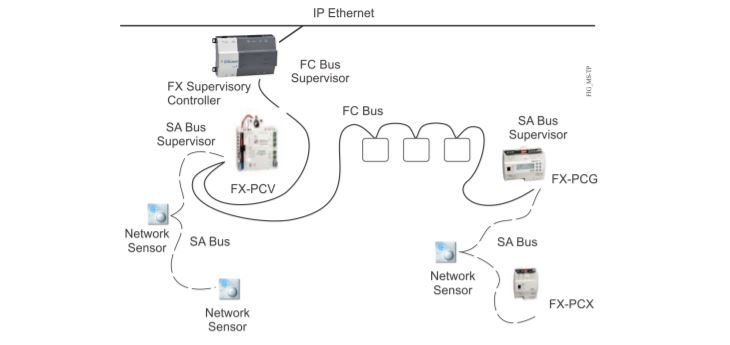
\includegraphics[width=1\textwidth]{2_MainMatter/Capitulo1/Imagenes/BACnet_MSTP_Johnson.JPG}
    \caption{Ejemplo de un bus de comunicaciones MS/TP\cite{MSTP}}
    \label{fig:BACnet_MSTP}
\end{figure}

El bus FC y el bus SA son redes de dispositivos conectados en cadena. Cada bus tiene solo un bus supervisor, dependiendo de qué controladores están conectados. En un bus local de FC, el supervisor de este es el controlador supervisor. En el bus SA local, el supervisor del bus es un controlador de campo.

El supervisor del bus se comunica con los dispositivos del bus supervisado y con los dispositivos del siguiente (nivel superior) bus en la red. El supervisor del bus FC generalmente inicia la comunicación en el FC bus o SA bus.

\section{Protocolo N2}
El bus de comunicación N2, es un protocolo desarrollado por Johnson Controls de red local que une controladores e interfaces al módulo de control de red(NCM \textit{network control module}). Este protocolo fue desarrollado principalmente para conectar los controladores desarrollados por Johnson Controls con sus dispositivos de campo.

\subsection{Estructura del sistema:}
El bus N2 utiliza un protocolo maestro/esclavo, en el cual es dispositivo maestro (NCM), inicia la comunicación con los dispositivos del bus N2. El bus N2 está conectado en cadena, en el que múltiples dispositivos están conectados en serie. A diferencia del protocolo BACnet, el bus N2 se comunica sólo entre el dispositivo maestro (NCM) y los dispositivos conectados en el mismo lazo. Sin embargo, para comunicarse entre dispositivos de más alto nivel, se utiliza el bus tipo N1 u otro protocolo de comunicación. Podemos observar un ejemplo de implementación de este bus en la Figura \ref{fig:N2}

\begin{figure}[H]
    \centering
    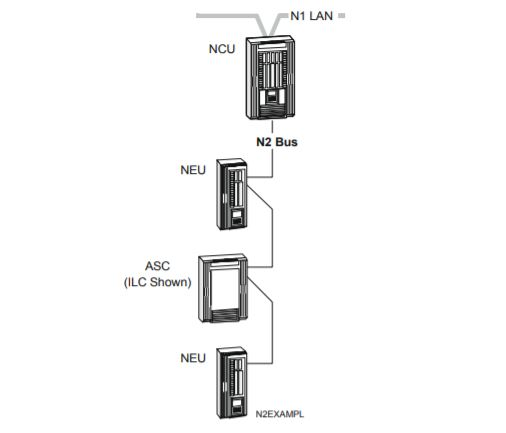
\includegraphics[width=0.60\textwidth]{2_MainMatter/Capitulo1/Imagenes/N2_Johnson.JPG}
    \caption{Ejemplo de un bus de comunicaciones N2\cite{N2}}
    \label{fig:N2}
\end{figure}
% ***************************************************************************************
% ************************************* CAPÍTULO II *************************************
% ***************************************************************************************
\chapter{DESCRIPCIÓN FUNCIONAL}
\thispagestyle{empty}

\section{Sistema de iluminación}
\subsection{Lógicas previas}
\section{Sistema de aire acondicionado}
\subsection{Lógicas previas}
\section{Sistema de bombeo primario variable}
\subsection{Lógicas previas}
\section{Estructura del espacio}

% ***************************************************************************************
% ************************************ CAPÍTULO III *************************************
% ***************************************************************************************
\chapter{ESTRUCTURA DE CONTROL}
\thispagestyle{empty}

\section{Estructura del sistema}
\subsection{Elementos de campo}
\subsection{Elementos de control}
\subsection{Elementos de gestión}
\subsection{Elementos de usuario}
% ***************************************************************************************
% ************************************* CAPÍTULO IV *************************************
% ***************************************************************************************
\chapter{** TITULO DEL CAPÍTULO 4 **}
\thispagestyle{empty}

** COLOQUE AQUÍ EL CONTENIDO RESPECTIVO DEL CAPÍTULO 4 **
% .
% .
% .
% \include{2_MainMatter/CapituloN/capN}

% ********************************** Conclusiones *******************************
% ***************************************************************************************
% ********************************** CONCLUSIONES ***************************************
% ***************************************************************************************
\chapter*{CONCLUSIONES Y RECOMENDACIONES}
\thispagestyle{empty}
\addcontentsline{toc}{chapter}{CONCLUSIONES Y RECOMENDACIONES}

\renewcommand{\thefigure}{C.\arabic{figure}}
\setcounter{figure}{0}

\epigraph{\flushright La web, tal como yo la imaginaba, todavía no la hemos visto. El futuro sigue siendo mucho más grande que el pasado}{\textit{Tim Berners-Lee}}

** COLOQUE AQUÍ SU CONTENIDO **

% *******************************************************************************
% ********************************** Back Matter ********************************
% *******************************************************************************

% ********************************** Referencias ********************************

\begin{spacing}{1}          % espaciado reglamentario
\printbibliography[heading=bibintoc, title=REFERENCIAS]
\end{spacing}

% ********************************** Apéndices ********************************
\appendix
% ***************************************************************************************
% ************************************** APÉNDICE A *************************************
% ***************************************************************************************
\chapter*{APÉNDICE A:\\ ** TITULO DEL APÉNDICE **}
\thispagestyle{empty}
\addcontentsline{toc}{chapter}{APÉNDICE A}

\renewcommand{\thefigure}{A.\arabic{figure}}
\setcounter{figure}{0}

\titlespacing\section{0pt}{12pt plus 4pt minus 2pt}{0pt plus 2pt minus 2pt}
\titlespacing\subsection{0pt}{12pt plus 4pt minus 2pt}{0pt plus 2pt minus 2pt}

** AQUÍ EMPIEZA EL APÉNDICE A **
% ***************************************************************************************
% ************************************** APÉNDICE B *************************************
% ***************************************************************************************
\chapter*{APÉNDICE B:\\ ** TITULO DEL APÉNDICE **}
\thispagestyle{empty}
\addcontentsline{toc}{chapter}{APÉNDICE B}

** AQUÍ EMPIEZA EL APÉNDICE B **
% ***************************************************************************************
% ************************************** APÉNDICE C *************************************
% ***************************************************************************************
\chapter*{APÉNDICE C:\\ ** TITULO DEL APÉNDICE **}
\thispagestyle{empty}
\addcontentsline{toc}{chapter}{APÉNDICE C}

** AQUÍ EMPIEZA EL APÉNDICE C **
% .
% .
% .
% \include{3_BackMatter/Apendices/apendiceN}

% *******************************************************************************
% *************************************** END ***********************************
% *******************************************************************************

\end{document}
